\documentclass[a4paper,11pt]{article}                                                                                                                                                            
\usepackage[ngerman]{babel}                                                                                                                                                                                 
\usepackage{listings}
\usepackage[dvipsnames]{xcolor}
\usepackage{graphicx}
\usepackage[belowskip=15pt, aboveskip=3pt]{caption}
\usepackage{mdframed}
\usepackage{enumerate}
\usepackage{enumitem}
\usepackage[left=3.5cm, right=3.5cm, includeheadfoot]{geometry}
\usepackage{wrapfig}
\usepackage{hyperref}
\usepackage{footnotebackref}
\usepackage{svg}
\usepackage{amsmath}

\definecolor{darkviolet}{rgb}{0.5,0,0.4} 
\definecolor{darkgreen}{rgb}{0,0.4,0.2} 
\definecolor{darkblue}{rgb}{0.1,0.1,0.9} 
\definecolor{darkgrey}{rgb}{0.5,0.5,0.5} 
\definecolor{lightblue}{rgb}{0.4,0.4,1} 


\begin{document}
\begin{titlepage}
	\centering
	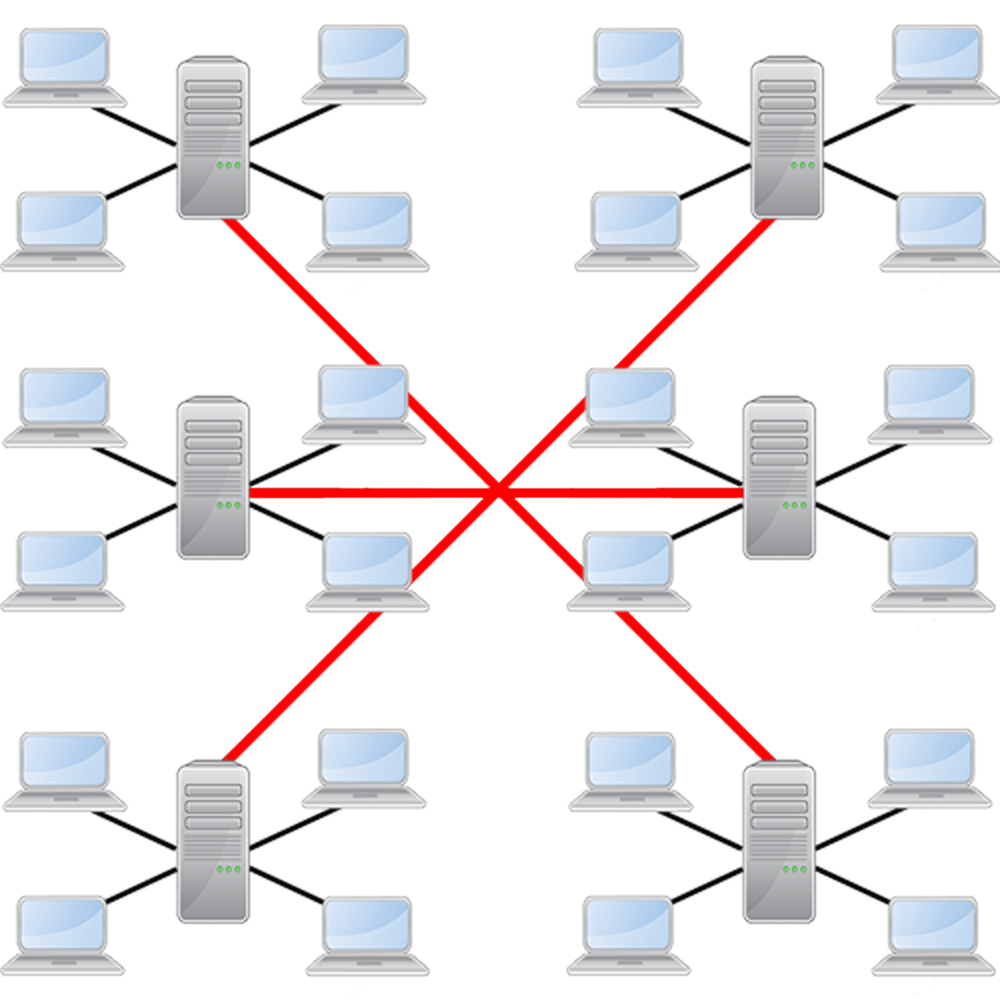
\includegraphics[width=0.15\textwidth]{Federation.png}\par\vspace{1cm} %https://datenschutzhelden.org/wp-content/uploads/2017/02/Federation.png
	{\scshape\LARGE Hochschule f\"ur Technik und Wirtschaft  \par}
	\vspace{1cm}
	{\scshape\Large Verteiltes Filesystem\par}
	\vspace{1.5cm}
	{\huge\bfseries Sitzungsprotokolle \par}
	\vspace{2cm}
	{\Large\itshape Wirth\par}
	\vfill

	\vfill
	% Bottom of the page
	{\large \par}
\end{titlepage}
\tableofcontents
\pagebreak

\section{Sitzungsprotokolle}
\subsection{24.10.2017}
TOP:
\begin{itemize}
\setlength\itemsep{0em}
\item Infrastruktur
	\begin{itemize}
	\setlength\itemsep{0.2em}
		\item WhatsApp, Discord, GitHub
		\item Versp\"atete Anmeldung an Herr Esch ging noch in der Stunde raus
	\end{itemize} 
\item Update Patrick Theis
	\begin{itemize}
		\item Um was gehts \"uberhaupt bzw. um was gings in VS1?
		\item Gruppenaustausch - Lessons Leraned
	\end{itemize}
\item Kommunikation
	\begin{itemize}
		\item Muss komplett neu geschrieben werden, da Umstieg von C-S auf P2P
	\end{itemize}
\item Recycling
	\begin{itemize}
		\item Die meisten Funktionen *m\"ussten* portierbar sein
		\item Infrastruktur bleibt bestehen
	\end{itemize}
\end{itemize}

\subsection{27.10.17:10:00- 13:00}
Struktureller Aufbau:
\begin{itemize}
\setlength\itemsep{0.2em}
\item Filesharing Service(Datei\"ubertragung)
\item Backup lokal auf PC (in Eigenverantwortuung)
\item evtl noch Logs senden-  Informationen über Sync Meldungen
\item Gui/Nogui
\item 2 Vlans (Wan) -Logische Verbindungen als mehrere Verbindungen
\item random link
\item Vertrag
\item P2P einlesen(pro/contra)
\item n\"achstes Treffen
\item Definition Ausfallsicherheit(Systemweit, aber nicht Rechnerweit)
\item Git /discord /wa
\item Stundenzettel
\item Prezi
\item trello?
\end{itemize}

Beschl\"usse bzw in n\"aherer Auswahl:
\begin{itemize}
\setlength\itemsep{0.2em}
\item Connection P2P neu (anpassen)
\item Explorervariante bleibt bestehen, XML bleibt bestehen, Funktionen bleiben erhalten
\item Python/Java
\item Nogui (Feature:Gui)
\item Nächstes Treffen Donnerstag ab Mittagspause Raum 5205 
\item Freitag 4. Stunde freihalten f\"ur Besprechung /Esch
\item Git aufr\"aumen nicht dazu gekommen
\end{itemize}
Fragen an Herrn Esch:
\begin{itemize}
\setlength\itemsep{0.2em}
\item Was ist mit 2 Verbindungen gemeint?
\end{itemize}

\subsection{Strategieplanung 4.11.17}
Basis: jxta "intern: jtags"
Kommunikation:
\begin{itemize}
\setlength\itemsep{0.2em}
\item beim Eintritt ins Netz -> Broadcast
\item bei Austritt aus dem Netz (unbeabsichtigt) ->timeout
\item FileServer!=FileSystem -> Frage an Esch: Was macht in dem Fall Sinn
\item Supernodes/Superpeers -benötigt?
\item Aufbauend auf p2p oder doppelte Arbeit?
\end{itemize}

\subsection{Planung mit Herrn Sauer 9.11.17}
keine nenneswerte Erfolge, Herr Sauer schliesst sich mit Herr Esch kurz und meldet sich dann wieder bei uns. Herr Sauer hatte Geburtstag.


\end{document}






